%!TEX root = ../thesis.tex
%*******************************************************************************
%****************************** Metodologia *********************************
%*******************************************************************************


\chapter{Metodología}\label{chap:metod}

Este trabajo aplica una metodología de \textbf{integración continua y desarrollo colaborativo} de acuerdo con los objetivos del proyecto SIOSE-INNOVA y con un marco de trabajo actual aplicado tanto en el Laboratorio de Geomática de la Universidad de Alicante como por otras empresas conocidas del sector (CARTO, Geographica, entre otros). En \citet{Zaragozi2017} se presentan distintos flujos de trabajo basados en esta metodología los cuales están muy relacionados con lo que se presenta en este capítulo.


\section{Integración continua y desarrollo colaborativo}

\begin{graybox}
\begin{itemize}
\item El trabajo colaborativo se ha coordinado utilizando \textit{Git} que es el sistema de \textbf{control de versiones} más popular de los últimos años (p.ej. utilizado en PostGIS, QGIS, CARTO y decenas de proyectos ESRI, entre muchos otros).
\item La \textbf{contenerización o \textit{dockers}} es una novedosa tecnología para la virtualización de software/servicios, frente a la virtualización de sistemas operativos (p.ej. máquinas virtuales). La orquestación de \textit{dockers} permite organizar complejos sistemas de información con muchas facilidades.
\item PostgreSQL/PostGIS es la \textit{geodatabase libre} más potente del mercado, destacando por sus opciones de \textbf{extensibilidad} (p.ej. PostGIS en sí misma es una extensión de PostgreSQL).
\end{itemize}
\end{graybox}

El trabajo colaborativo ha sido uno de los aspectos más fundamentales para la coordinación del desarollo de la extensión \textit{pg\_landmetrics} en este trabajo donde se ha aplicado un procedimiento de integración continua y desarrollo colaborativo.

En la subsección \ref{subsec:control} se describe el sistema de control de versiones más popular de los últimos años entre usuarios y que se ha aplicado en este trabajo. A continuación, en la subsección \ref{subsec:conten-orquest} se presentan los servicios de contenerización o \textit{dockers} que se han utilizado para la virtualización del software/servicios necesarios para el desarrollo de la extensión, y la orquestación de éstos. En la subsección \ref{subsec:exten} se muestra la geodatabase más potente destacada por su extensibilidad que se ha aplicado para el manejo y gestión de la base de datos del SIOSE. Finalmente, en la subsección \ref{subsec:aplic} se describen las aplicaciones que se han utilizado para diversos procesos de la metodología.

Es importante destacar que en esta sección se presenta el procedimiento que se ha seguido de forma periódica y diaria en este trabajo desde la integración continua y el desarrollo colaborativo.


\subsection{Control de versiones}\label{subsec:control}

El control de versiones es la gestión de los cambios que se realizan sobre un archivo o conjunto de archivos en un repositorio y que se utiliza para controlar las versiones del código de fuente, de modo que se puedan recuperar versiones anteriores en un momento específico. Un repositorio es donde se almacenan todos los datos actualizados y los registros históricos de los cambios realizados, principalmente en un servidor.

En este caso, se trabaja de forma colaborativa donde cada usuario modifica desde su máquina local, comparte los cambios y luego el sistema de control combina las modificaciones. En este trabajo se ha utilizado los siguientes sistemas de control de versiones:

\begin{itemize}
\item\textbf{Git}\footnote{\url{https://git-scm.com/}} es un sistema de control para el mantenimiento de versiones de código fuente de archivos. Es el más popular de los últimos años y es utilizado por muchos proyectos como por ejemplo PostGIS, QGIS, CARTO y decenas de proyectos de ESRI, entre otros más. Para la actualización de archivos desde la máquina local se utilzan formas verbales como \textit{pull}, \textit{push}, \textit{add}, \textit{commit}, \textit{clone}, entre otros.
\item\textbf{GitHub}\footnote{\url{https://github.com/}} es una plataforma de desarrollo colaborativo que alberga proyectos y almacena de forma pública el código fuente utilizando el sistema de control de versiones de \textit{Git}.
\end{itemize}

Todos los archivos que se han generado para la extensión \textit{pg\_landmetrics} se encuentran en el repositorio de este trabajo\footnote{\url{https://github.com/andrearosado/pg_landmetrics}} y en el repositorio proyecto SIOSE-INNOVA\footnote{\url{https://github.com/siose-innova/pg_landmetrics}}.

Uno de los procesos de integración continua y desarrollo colaborativo que se ha realizado es la actualización de ficheros de la extensión \textit{pg\_landmetrics} al repositorio del trabajo (ver la figura \ref{fig:diary}). El procedimiento consistía en que el usuario ejecutaba el comando \textit{pull} desde la máquina local cuando el sistema de ficheros de la extensión no estaba actualizado y éste se encargaba de obtener la última versión. Este paso es opcional si el sistema de ficheros tenía la última versión y no era necesario ejecutar la anterior instrucción. Una vez el usuario recibía un mensaje de notificación de que su sistema de fichero estaba actualizado, se procedía a editar los archivos. Cuando la edición finalizaba, el usuario se encargaba de transmitir todas las modificaciones realizadas a partir de los comandos \textit{add} y \textit{commit}, y a continuación recibía un mensaje de notificación con un \textit{hash} (identificador único) por cada cambio que se había realizado en el proceso. Finalmente, el usuario desde la máquina local subía esta última versión del sistema de ficheros de la extensión al repositorio del trabajo a partir del comando \textit{pull} y así obtener una nueva versión actualizada.

\begin{figure}
\begin{center}
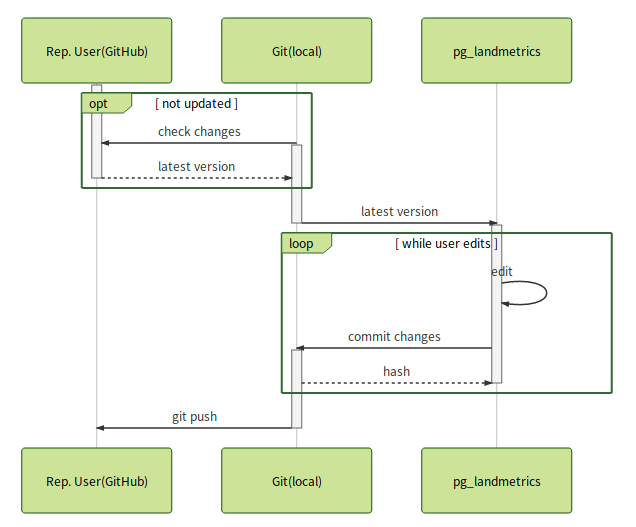
\includegraphics[width=0.9\textwidth]{Metodologia/Figs/diary.png}
\caption{Flujo de proceso de actualización de ficheros. \label{fig:diary}}
\end{center}
\end{figure}

Otro de los procesos de integración continua y desarrollo colaborativo que se ha realizado es la actualización de la extensión entre el repositorio del trabajo y el repositorio \textit{upstream} del proyecto SIOSE-INNOVA (ver la figura \ref{fig:pullrequest}). Una de las primeras tareas era realizar un \textit{fork}, es decir, una copia de todos los ficheros del repositorio \textit{upstream} a un nuevo repositorio de este trabajo. La ventaja es que si en cualquier momento el repositorio del usuario sufría algún contratiempo, se podía volver a realizar un \textit{fork} del repositorio \textit{upstream}. Lo mismo ocurre cuando en nuestra máquina local se tenía el sistema de ficheros de la extensión a partir del comando \textit{clone}. Éste último comando era ejecutado solamente cuando en la máquina local no existía el sistema de ficheros de \textit{pg\_landmetrics}. A continuación se realizaba o no un chequeo de la última versión de la extensión, como se realizaba en el anterior proceso. A partir de aquí, se inicia el trabajo colaborativo entre usuarios y repositorios. En este caso, se vuelve a repetir las mismas acciones de edición y actualización de archivos como en el anterior proceso. Una vez se tenían todos los ficheros de la extensión con una nueva última versión, el usuario enviaba una petición al repositorio \textit{upstream} para emparejar ambos repositorios a través de la función \textit{pull request} que se encuentra en la plataforma de \textit{GitHub}. Si la petición era aceptada por el personal encargado del repositorio \textit{upstream}, se ejecutaba el comando \textit{merge} (unión) y se recibía una notificación de sincronización completada. Finalmente los repositorios quedaban sincronizados y los ficheros con la última versión. Se volvían a subir los cambios al repositorio del trabajo y se recibía una notificación de que los cambios habían sido correctos.

\begin{figure}
\begin{center}
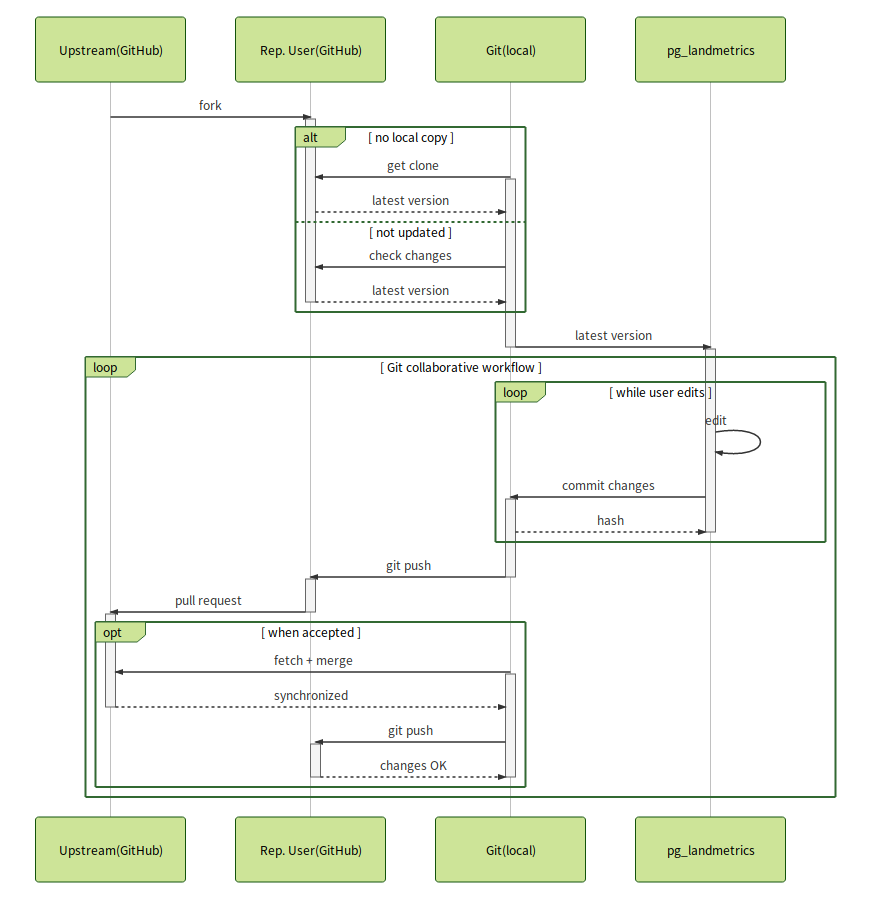
\includegraphics[width=0.9\textwidth]{Metodologia/Figs/pullrequest.png}
\caption{Flujo de proceso de trabajo colaborativo entre repositorios. \label{fig:pullrequest}}
\end{center}
\end{figure}


\subsection{Contenerización y orquestación de servicios}\label{subsec:conten-orquest}

La contenerización o \textit{docker} es una novedosa tecnología que aporta portabilidad y que virtualiza softwares y servicios frente a la virtualización de sistemas operativos completos como son por ejemplo las máquinas virtuales. Las herramientas de \textit{docker} ofrecen las funciones de construir (\textit{build}), subir o iniciar (\textit{up}) y bajar o detener (\textit{down}) los contenedores que son como ''cajas'' donde se almacena lo esencial para ejecutar un determinado software o servicio. En cuanto a la orquestación de contenedores, éste permite organizar complejos sistemas de información con muchas facilidades. En este trabajo se ha utilizado las siguientes herramientas:

\begin{itemize}
\item\textbf{Docker}\footnote{\url{https://www.docker.com/}}: es un proyecto de código abierto que proporciona el despliegue y movilidad de contenedores a través de la nube. Permite autosuficiencia entre las aplicaciones y la infraestructura y los desarrolladores y operaciones para crear un modelo colaborativo e innovador.
\item\textbf{Docker Hub}\footnote{\url{https://hub.docker.com/}}: es un servicio en la nube que permite vincular repositorios y crear y almacenar sus imágenes. Es una plataforma que centraliza y distribuye las imágenes en contenedores, además de auomatización en el proceso de desarrollo.
\item\textbf{Docker-compose}: es un fichero de configuración que despliega todos los servicios que sean necesarios durante el desarrollo de manera rápida y eficaz.
\end{itemize}

Finalmente, otro de los procesos de integración continua y desarrollo colaborativo que se ha realizado es el funcionamiento de los \textit{dockers} y extensiones a la hora de implementar y desarrollar las funciones en la extensión \textit{pg\_landmetrics} (ver la figura \ref{fig:ci}). Desde el punto de vista del usuario, se ejecutaba el comando \textit{docker-compose build} si la extensión había sido modificada. En el caso de que no lo estuviera y no fuera necesario volver a construir el \textit{docker-compose}, solamente era necesario ejecutar el comando \textit{docker-compose up} para iniciarlo. A partir de aquí, el \textit{docker-compose} orquestaba y se ocupaba de lanzar dos contenedores: PostgreSQL/PostGIS y PgAdmin. Una vez han sido lanzados dichos contenedores y se han recibido las notificaciones de que la conexión había sido satisfactoria, el usuario realizaba consultas a los contenedores. A continuación, los contenedores realizaban consultas entre ambos y luego se enviaban al usuario los resultados de las consultas acompañado de una vista previa de ellos. Cuando ya eran adquiridos todos los resultados deseados, se ejecutaba el comando \textit{docker-compose down} para que el \textit{docker-compose} dejase de funcionar y el usuario recibiese una notificación por parte de este actor de que había dejado de ''funcionar'' sin ningún problema.

\begin{figure}
\begin{center}
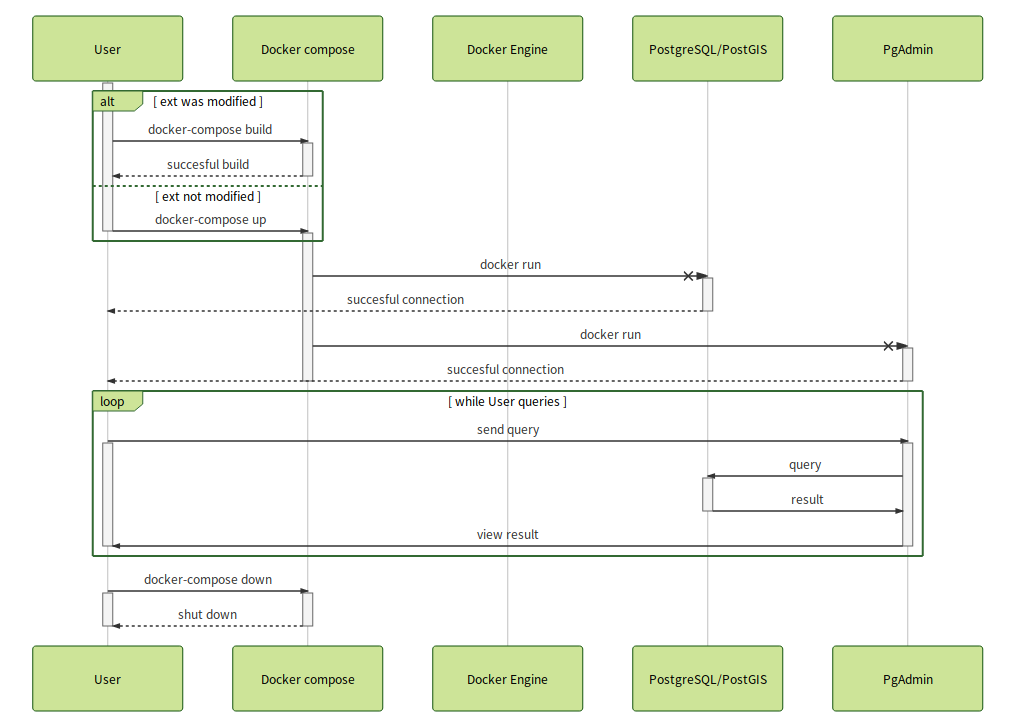
\includegraphics[width=\textwidth]{Metodologia/Figs/ci.png}
\caption{Flujo de proceso de integración continua. \label{fig:ci}}
\end{center}
\end{figure}


\subsection{Extensibilidad}\label{subsec:exten}

La extensibilidad es la fácil adaptación del software a los nuevos cambios realizados en su especificación. Para ello se utiliza un \textit{makefile} que es un fichero que se encarga de organizar todo el código compilado de todos los softwares necesarios para el desarrollo. Este fichero tiene la capacidad de ampliar las funcionalidades de cualquier aplicación. En este trabajo se ha utilizado la siguiente extensión:

\begin{itemize}
\item\textbf{PostgreSQL/PostGIS}: es la geodatabase libre más potente del mercado diseñada para ser extensible. PostGIS, como extensión, habilita y agrega soporte a objetos espaciales a la base de datos relacional de PostgreSQL.
\end{itemize}


\subsection{Aplicaciones}\label{subsec:aplic}

Para la elaboración del conjunto de datos que se han utilizado en este trabajo y las consultas y funciones que se han desarrollado para la extensión \textit{pg\_landmetrics}, se han utilizado las siguientes aplicaciones:

\begin{itemize}
\item\textbf{PgAdmin4}\footnote{\url{https://www.pgadmin.org/}}: es una plataforma que administra, gestiona y desarrolla código abierto en bases de datos PostgreSQL. En la figura \ref{fig:carga} se muestra el interfaz en el cual se ha trabajado.
\item\textbf{QGIS 2.18}\footnote{\url{https://www.qgis.org/es/site/}}: es una aplicación de escritorio SIG, de código abierto, que analiza, maneja y opera con datos como \textit{raster/vector} y bases de datos. Además, facilita la conexión entre bases de datos espaciales como PostGIS.
\end{itemize}

\begin{figure}
\begin{center}
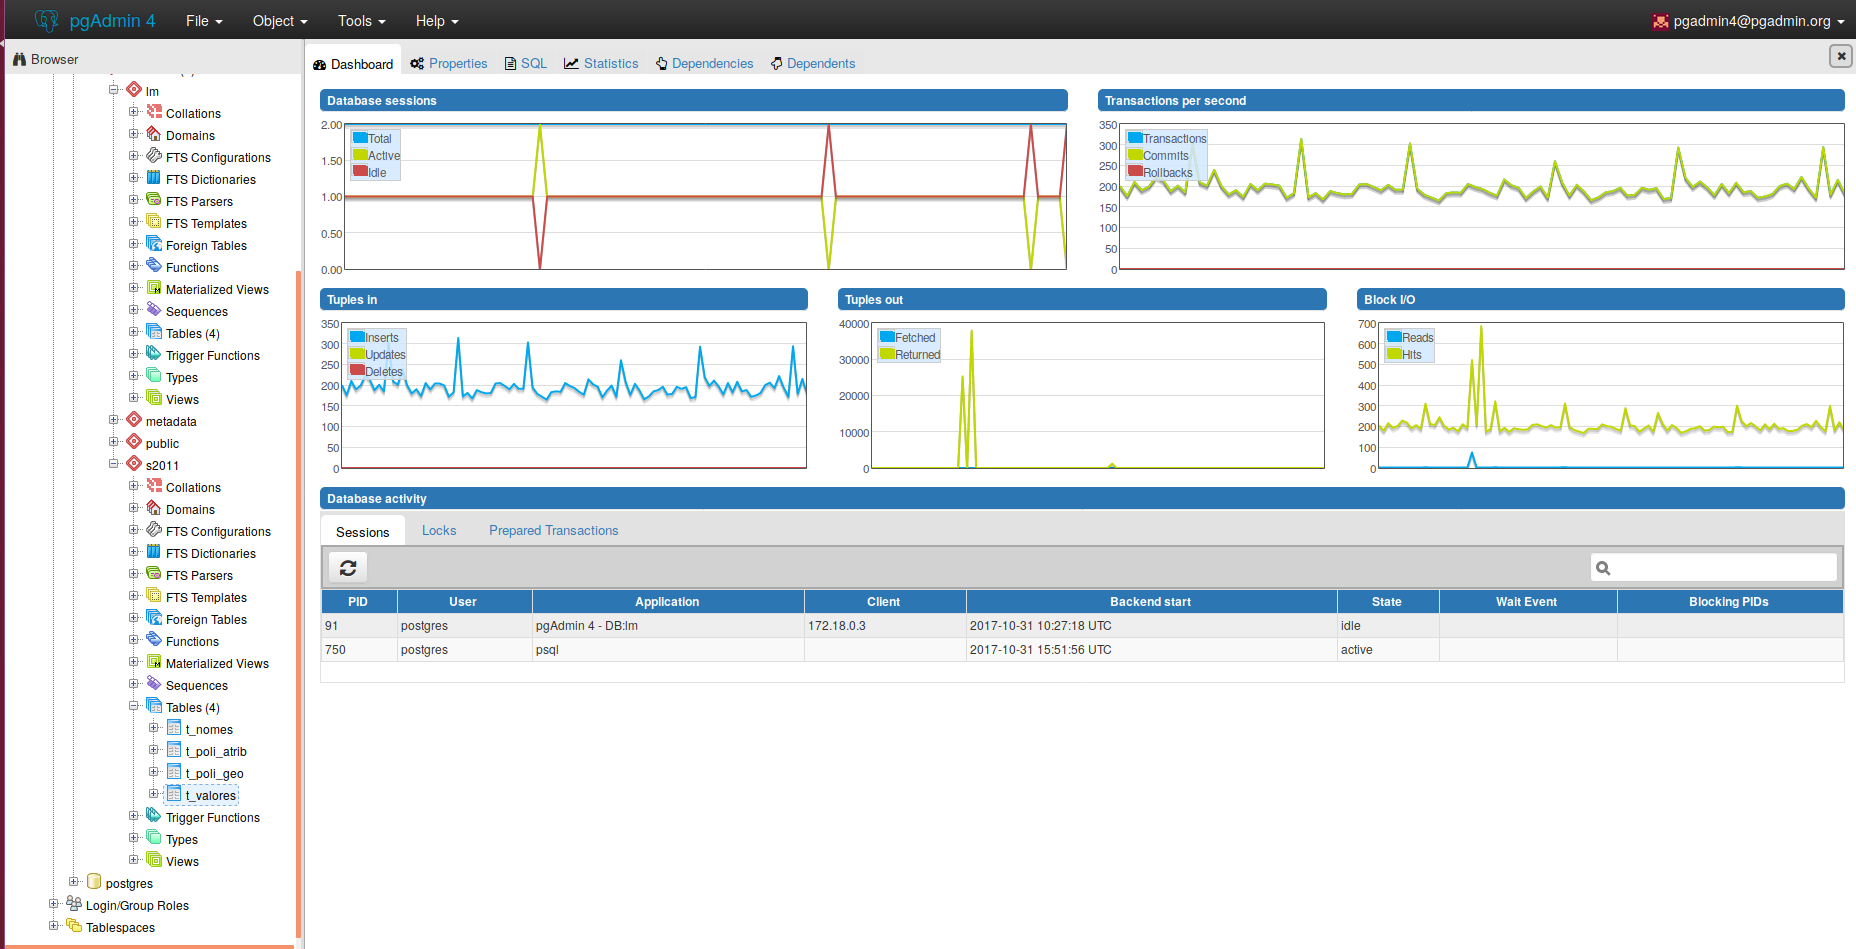
\includegraphics[width=\textwidth]{Metodologia/Figs/carga-siose-2011.png}
\caption{Flujo de proceso de integración continua. \label{fig:carga}}
\end{center}
\end{figure}


\section{Conjunto de datos}

\begin{graybox}
\begin{itemize}
\item En este trabajo se han utilizado dos conjuntos de datos, \textbf{un paisaje de ejemplo y el SIOSE de 2011 completo}, para poner a prueba la extensión \textit{pg\_landmetrics} propuesta en los objetivos.
\item Para demostrar que la \textbf{extensión} es \textbf{escalable}, se han utilizado distintas escalas de referencia a partir de \textit{grids}.
\end{itemize}
\end{graybox}

Para someter a prueba la extensión \textit{pg\_landmetrics} se han utilizados dos conjuntos de datos: un paisaje de ejemplo y el SIOSE de 2011.

El \textbf{paisaje de ejemplo} se ha utilizado para comprobar si las métricas de paisaje funcionan correctamente desde PgAdmin como también en QGIS. La escala de referencia es 1:50.000 en dos sistemas geodésicos de referencia: European Terrestrial Reference System 1989 (ETRS89) y World Geodetic System 84 (WGS84), ya que las métricas no se calculan igual si son proyectadas (\textit{geometry}) o son coordenadas esféricas (\textit{geography}). 

En este conjunto de datos hay un total de 51 polígonos que se han digitalizado a partir de las herramientas de geoproceso y edición avanzada mediante la aplicación de QGIS. En total hay 8 categorías de cobertura de suelo donde a cada polígono le corresponde un tipo de categoría representada por un color (ver figura \ref{fig:zona_andrea}). Se han definido los colores a partir de los 147 que presenta Scalable Vector Graphics (SVG) Specification\footnote{\url{http://www.december.com/html/spec/colorsvg.html}} además del apoyo de la clasificación de color que especifica el \textit{Corine Land Cover (CLC)}.

\begin{figure}
\begin{center}
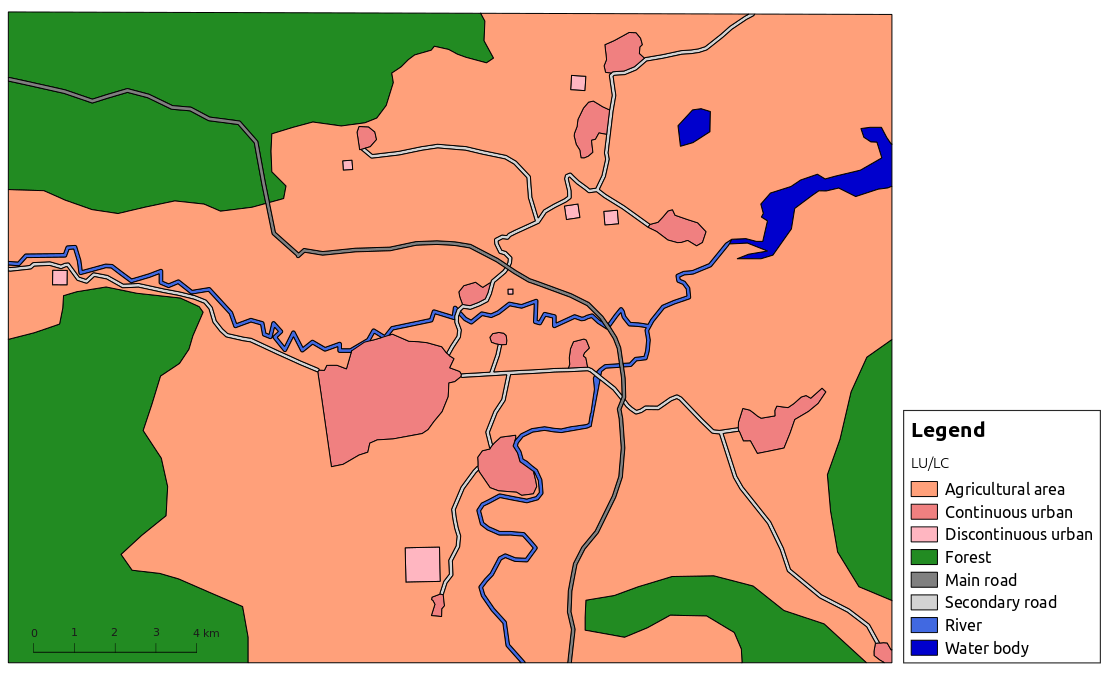
\includegraphics[width=\textwidth]{Metodologia/Figs/zona_andrea.png}
\caption{Cobertura del suelo del paisaje de ejemplo. \label{fig:zona_andrea}}
\end{center}
\end{figure}

Una vez se han comprobado que las métricas de paisaje funcionan correctamente, el segundo conjuntos de datos que se ha utilizado para obtener los resultados es el \textbf{SIOSE 2011}, datos que se han obtenido a partir del equipo técnico del SIOSE que colabora en el proyecto SIOSE-INNOVA. 

Esta base de datos tan voluminosa se componen de 4 tablas. En la tabla de datos \texttt{t\_nomes} se encuentran todas las nomenclaturas de cada polígono, en \texttt{t\_poli\_atrib} todos los atributos de los polígonos como por ejemplo el código multietiqueta de clasificación del SIOSE o de clasificación de las distintas nomenclaturas (iberpix, perfil ambiental, toponimia, \textit{Corine Land Cover}, etc.), en cuanto a la tabla \texttt{t\_poli\_geo} ofrece la geometría de cada uno de los 2.562.800 de polígonos en total y finalmente, en la tabla \texttt{t\_valores} calculos estádisticos como por ejemplo la superficie en hectáreas.

Como se menciona en la sección \ref{sec:siose}, los polígonos del SIOSE presentan una \textit{cobertura simple} o una \textit{cobertura compuesta}. Dentro de esta última cobertura se encuentran las coberturas no predefindidas, es decir, que un mismo polígono puede contener varías coberturas de suelo. A raíz de esta característica, se ha realizado una reclasificación de los polígonos a partir de la cobertura prevalente que presenta la jerarquización de la clasificación de los usos y coberturas del suelo del SIOSE. Con ello se ha obtenido una nueva tabla con 85 coberturas prevalentes asignadas a cada uno de los polígonos que se encuentran en la tabla \texttt{t\_poli\_geo}. Para que las consultas sean más rápidas entre las distintas tablas se han generado índices para indexar los datos de cada una de las tablas. 

Una vez se han reclasificado todos los polígonos del SIOSE 2011, se han obtenido \textbf{\textit{grids}} (cuadrículas cartográficas) para el cálculo de métricas del paisaje en distintas escalas de referencia, a través del Centro de Descargas del Instituto Geográfico Nacional (CNIG)\footnote{\url{http://centrodedescargas.cnig.es/CentroDescargas/index.jsp}}. 

A partir del grid 1:500.000 se han escogido dos celdas de las zonas de estudio en las cuales se han calculado algunas métricas de paisaje. Estas dos zonas comprenden en su mayor parte a la provincia de Alicante y a la provincia de Zaragoza, y los alrededores de cada una. El motivo de por qué se han escogido estas dos zonas es por hacer referencia al lugar donde se han realizado las prácticas de empresa y dónde se ha impartido el \textit{máster}.

Dado que ya se han escogido las zonas de estudio, a continuación se han seleccionado y extraído todas aquellas celdas que comprenden las dos celdas de las áreas de estudio con escala de referencia 1:25.000, 1:50.000 y 1:100.000. A partir de éstas se han realizado todos los resultados que pueden consultarse en el capítulo \ref{chap:result}.


\section{Selección de métricas}

\begin{graybox}
\begin{itemize}
\item El número potencial de métricas del paisaje es indeterminado y depende de muchos factores (p.ej. objetivos del estudio, modelos de datos como \textit{raster/vector} o en red, niveles de agregación y/o escala, etc).
\item Resulta esencial determinar unas \textbf{métricas representativas} para esta primera propuesta.
\end{itemize}
\end{graybox}

Como se indica en la sección \ref{sec:metrica}, existen cientos de métricas de paisaje que no siempre tienen significado para todas las aplicaciones de estudio ya que dependen de muchos factores, como por ejemplo los objetivos del estudio, el modelo de datos, la escala, nivel de agregación etc. Por este mismo motivo y según los objetivos específicados en este trabajo y en el proyecto SIOSE-INNOVA, se han seleccionado unas determinadas métricas de paisaje para esta primera propuesta de extensión.

En la tabla \ref{tab:listmetricas} se aprecian las métricas, acompañadas por su abreviatura, que se han escogido divididas en tres niveles de agregación: a nivel de polígono (\textit{patch}), nivel de categoría (\textit{class}) y nivel de paisaje (\textit{landscape}). Para ello se ha seleccionado un número equitativo entre los niveles de agregación. Además, se han querido escoger algunas métricas que calculen operaciones simples como por ejemplo el área o perímetro, y por otro lado, métricas cuyos cálculos sean más complejos como por ejemplo la distancia del vecino más próximo o la densidad, entre otros.

% Please add the following required packages to your document preamble:
% \usepackage{multirow}
\begin{table}[]
\centering
\caption{Métricas de paisaje disponibles en la extensión.}
\label{tab:listmetricas}
\begin{tabular}{lll}
\hline
\textbf{Nivel}             & \textbf{Métrica}                     & \textbf{Abreviatura} \\ \hline
\multirow{8}{*}{Patch}     & Patch Area                           & AREA                 \\
                           & Patch Perimeter                      & PERIM                \\
                           & Perimeter-Area-Ratio                 & PARA                 \\
                           & Shape Index                          & SHAPE                \\
                           & Core Area                            & CORE                 \\
                           & Number of Core Areas                 & NCORE                \\
                           & Core Area Index                      & CAI                  \\
                           & Euclidean Nearest Neighbour Distance & ENN                  \\ \hline
\multirow{8}{*}{Class}     & Total (Class) Area                   & CA                   \\
                           & Percentage of Landscape              & PLAND                \\
                           & Total Edge                           & TE                   \\
                           & Edge Density                         & ED                   \\
                           & Total Core Area                      & TCA                  \\
                           & Core Area Percentage of Landscape    & CPLAND               \\
                           & Number of Patches                    & NP                   \\
                           & Patch Density                        & PD                   \\ \hline
\multirow{9}{*}{Landscape} & Total Area                           & TA                   \\
                           & Total Edge                           & TE                   \\
                           & Edge Density                         & ED                   \\
                           & Number of Patches                    & NP                   \\
                           & Patch Density                        & PD                   \\
                           & Patch Richness                       & PR                   \\
                           & Patch Richness Density               & PRD                  \\
                           & Shannon's Diversity Index            & SHDI                 \\
                           & Simpson's Diversity Index            & SHIDI                \\ \hline
\end{tabular}
\end{table}


\section{Implementación/desarrollo de funciones en PostgreSQL}

\begin{graybox}
\begin{itemize}
\item Los desarrollos en PostgreSQL se pueden realizar en lenguajes de programación como ANSI C, SQL y/o distintos lenguajes procedurales (p.ej. PLpgSQL, PL/R, PL/Python, entre muchos otros), \textbf{dependiendo de las necesidades}.
\end{itemize}
\end{graybox}


\lstset{caption=Crear una función para calcular el IDW (I),label= IDW1}
\begin{SQL}
SELECT St_Area(geom)/10000 FROM sample_patches_25830;
SELECT St_Area(geom)/10000 FROM sample_patches_4326;
\end{SQL}

\lstset{caption=Crear una función para calcular el IDW (I),label= IDW1}
\begin{SQL}
SELECT SUM(St_Area(geom))/10000, category FROM sample_patches_25830 GROUP BY category;
SELECT SUM(St_Area(geom))/10000, category FROM sample_patches_4326 GROUP BY category;
\end{SQL}

\lstset{caption=Crear una función para calcular el IDW (I),label= IDW1}
\begin{SQL}
SELECT SUM(St_Area(geom)) FROM sample_patches_25830;
SELECT SUM(St_Area(geom)) FROM sample_patches_4326;
\end{SQL}


\lstset{caption=Crear una función para calcular el IDW (I),label= IDW1}
\begin{SQL}
SELECT St_Distance(p1.geom, p2.geom) 
FROM sample_patches_25830 AS p1, sample_patches_25830 AS p2
WHERE p1.id = 1 AND p1.id <> p2.id AND p2.category= "category"
ORDER BY St_Distance (p1.geom, p2.geom)
LIMIT 1;

SELECT St_Distance(p1.geom, p2.geom) 
FROM sample_patches_4326 AS p1, sample_patches_4326 AS p2
WHERE p1.id = 1 AND p1.id <> p2.id AND p2.category= "category"
ORDER BY St_Distance (p1.geom, p2.geom)
LIMIT 1;
\end{SQL}

\lstset{caption=Crear una función para calcular el IDW (I),label= IDW1}
\begin{SQL}
SELECT SUM(St_Area(St_Buffer(geom, -100)))/10000 FROM sample_patches_25830 GROUP BY category;
SELECT SUM(St_Area(St_Buffer(geom, -100)))/10000 FROM sample_patches_4326 GROUP BY category;
\end{SQL}

\lstset{caption=Crear una función para calcular el IDW (I),label= IDW1}
\begin{SQL}
SELECT SUM(St_Perimeter(geom)/St_Area(geom))*10000 FROM sample_patches_25830;
SELECT SUM(St_Perimeter(geom)/St_Area(geom))*10000 FROM sample_patches_4326;
\end{SQL}


\lstset{caption=Crear una función para calcular el IDW (I),label= IDW1}
\begin{SQL}
SELECT (p_corearea(geom, 50)).value FROM sample_patches_25830;
SELECT (p_corearea(geom, 50)).value FROM sample_patches_4326;
\end{SQL}

\lstset{caption=Crear una función para calcular el IDW (I),label= IDW1}
\begin{SQL}
SELECT c_totalarea(geom,category) FROM sample_patches_25830;
SELECT c_totalarea(geom,category) FROM sample_patches_4326;
\end{SQL}



\section{Documentación de la extensión}

\begin{graybox}
\begin{itemize}
\item Una parte fundamental de esta metodología es la \textbf{documentación} del desarrollo y uso de la extensión. 
\item Una buena documentación con ejemplos facilitará el cálculo de métricas del paisaje en grandes repositorios, \textbf{sobretodo para aquellos usuarios con menos experiencia} en PostgreSQL/PostGIS.
\end{itemize}
\end{graybox}

La documentación del desarrollo y uso de la extensión es una de las partes más importante de la metodología de este trabajo. Una buena documentación facilita la aplicación de todas las medidas necesarias para llevar a cabo el funcionamiento de la extensión a cualquier usuario, sobretodo a aquellos menos expertos en la materia. Así pues, se han aplicado los siguientes lenguajes de marcado:

\begin{itemize}
\item\textbf{Markdown}\footnote{\url{https://github.com/adam-p/markdown-here/wiki/Markdown-Cheatsheet}} es un lenguaje ligero que permite una escritura sencilla y de fácil lectura usando texto plano. Se ha utilizado para documentar el usp de la extensión.
\item\textbf{TeX}\footnote{\url{https://www.latex-project.org/}} es el lenguaje que se utiliza en el sistema de textos LaTeX y que crea documentos con una alta calidad tipográfica. Desde hace tiempo este lenguaje se emplea por un gran número de usuarios para escribir artículos o libros científicos. Para trabajar con este lenguaje, se ha utilizado la aplicación Texmaker y se ha utilizado para escribir este trabajo.
\item\textbf{Scalable Vector Graphics (SVG)}\footnote{\url{https://www.w3schools.com/graphics/svg_intro.asp}} es un lenguaje capaz de crear gráficos basados en vectores escalables de alta calidad de resolución. A partir de este lenguaje se ha desarrollado una función capaz de representar gráficos vectoriales a partir de las geometrías de cualquier geodatabase (ver en el anexo \ref{anex:svg}).
\item\textbf{Mermaid}\footnote{\url{https://mermaidjs.github.io/}} es un lenguaje que genera gráficos a partir de texto mediante JavaScript. Se han generado desde diagramas de flujo hasta diagramas de secuencia y de Gantt.
\end{itemize}
